\documentclass[10pt,a4paper]{article}
\usepackage[margin=2.1cm]{geometry}
\usepackage{amsmath,amssymb,bm}
\usepackage{graphicx,booktabs,xcolor,enumitem,hyperref}
\hypersetup{colorlinks,linkcolor=blue!50!black,urlcolor=blue!50!black}
\newcommand{\kc}{\kappa_2}
\newcommand{\ka}{\kappa_1}
\newcommand{\note}[1]{\par\smallskip\noindent\colorbox{gray!12}{\parbox{\dimexpr\linewidth-2\fboxsep}{\small #1}}\par\smallskip}
\newcommand{\evd}[1]{\textsf{\small[#1]}}
\newcommand{\simple}[1]{\par\noindent\textbf{In simple words:} #1\par\smallskip}
\title{TOP-Q --- Day 4 worked notes\\[2pt]\large Monte Carlo study 1: how much does the mode's propagation constant move?}
\author{PH 5110 term paper --- Kotapati Kishore (EE26E016)}
\date{31 October 2026}
\begin{document}\sloppy\maketitle

\note{Everything in Sections 2--5 is a \textbf{numerical simulation} \evd{Simulated}, not a measurement. Arrays T and D are the Day-3 designs ($M=41$, $\ka/\kc=1/3$, matched IPR $=0.656$). Units: $b$ and $\sigma_\beta$ in units of $\kc$; $\sigma_\kappa$ is dimensionless.\\
\textbf{Schedule:} today is 31 Oct; Day 4 was planned for 25 Oct. Section 7 gives the revised plan to 11 Nov.}

\tableofcontents

%=====================================================================
\section{What a Monte Carlo experiment is, and how ours is set up}
%=====================================================================
\simple{we cannot fabricate thousands of chips, so we let the computer ``make'' 2000 random chips for each setting, each with slightly different errors, and look at how much the result varies from chip to chip.}

\begin{tabular}{@{}p{0.27\linewidth}p{0.66\linewidth}@{}}\toprule
Setting & Choice and reason\\\midrule
Samples per point & $N=2000$. The statistical error of a standard deviation is about $1/\sqrt{2N}\approx1.6\%$.\\
Disorder strengths & 11 values of $\sigma$ from 0.003 to 0.3, evenly spaced on a log scale, so we see both the ``small error'' regime (where first-order theory should hold) and the ``large error'' regime.\\
Disorder types & coupling (gap errors), on-site (width/height errors), width model with $\sigma_\beta=\sigma_\kappa$ (Day 3).\\
Random numbers & every sample $s$ uses \texttt{SeedSequence([seed, s])}; each block of the study has its own documented seed. Rerunning gives identical numbers \evd{Verified-by-test}.\\
Which mode? & For each random chip we pick the eigenmode that \textbf{looks most like the clean mode} (largest overlap $|\langle\psi_0|\psi\rangle|^2$). This is a choice; Section 4.2 shows where it matters.\\
Error bars & 95\% bootstrap confidence intervals: resample the 2000 values 1000 times and look at how much the std changes.\\
Run time & about 41 s on one CPU core (whole study).\\\bottomrule
\end{tabular}

\textbf{Convergence check} \evd{Simulated}. T under on-site disorder, $\sigma=0.05$: std$(\delta b)$ = 0.0404, 0.0412, 0.0396, 0.0390, 0.0406, 0.0406 for $N$ = 125, 250, 500, 1000, 2000, 4000. The confidence interval shrinks from $\pm9\%$ to $\pm2\%$ and the value settles at $0.0406\approx0.81\times0.05$. $N=2000$ is enough.

%=====================================================================
\section{Results: the spread of $b$}
%=====================================================================
\begin{figure}[t]\centering
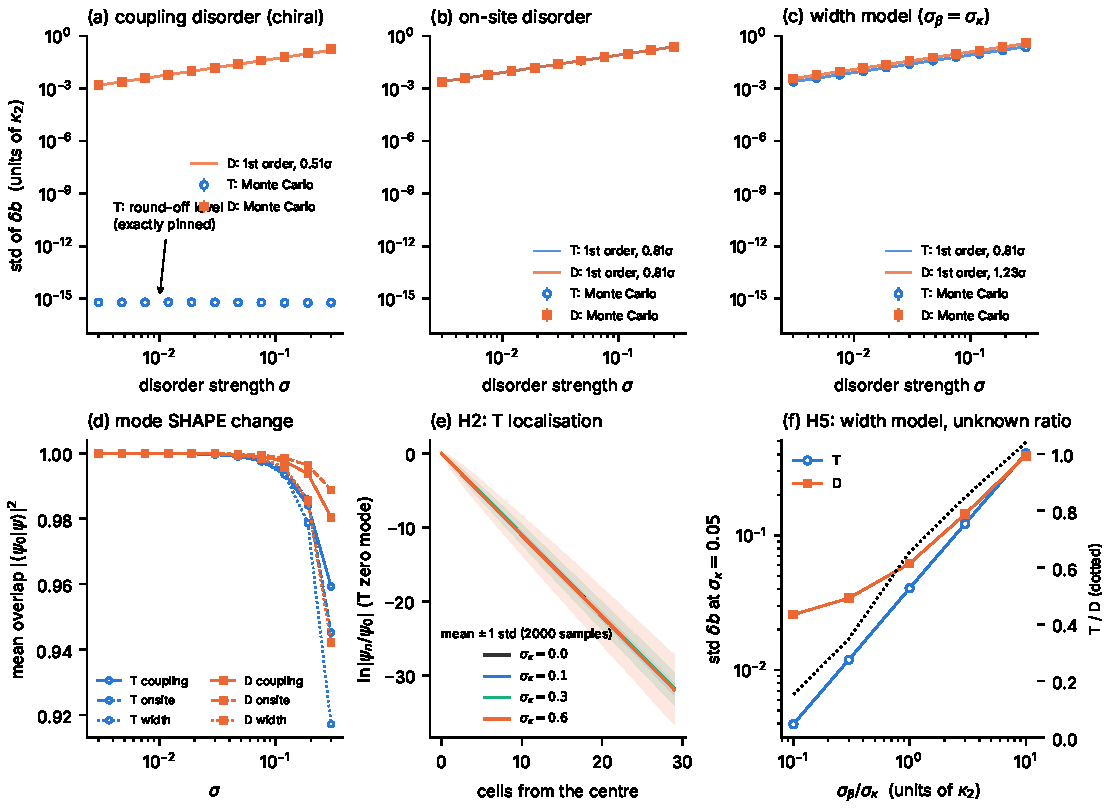
\includegraphics[width=\linewidth]{../../figures/fig_mc_eigen.pdf}
\caption{Generated by \texttt{scripts/day4\_mc\_eigen.py} from \texttt{data/day4\_mc\_eigen.npz}. (a)--(c) Spread of $\delta b$ vs.\ disorder strength (points: Monte Carlo, 2000 samples, 95\% bootstrap bars; lines: first-order prediction from Day 3). In (b) the T and D curves lie on top of each other. (d) Mean overlap of the disordered mode with the clean one. (e) Decay of the exact T zero mode under coupling disorder (mean $\pm$1 std of $\ln|\psi_n/\psi_0|$). (f) Width model at $\sigma_\kappa=0.05$ for different $\sigma_\beta/\sigma_\kappa$.}
\label{fig:mc}
\end{figure}

\begin{tabular}{@{}lccc@{}}\toprule
std$(\delta b)/\sigma$ for small $\sigma$ ($\le0.03$) & coupling & on-site & width ($\sigma_\beta=\sigma_\kappa$)\\\midrule
T predicted / \textbf{measured} & 0 / $\mathbf{\sim10^{-15}}$ & 0.810 / \textbf{0.815} & 0.810 / \textbf{0.814}\\
D predicted / \textbf{measured} & 0.506 / \textbf{0.508} & 0.810 / \textbf{0.805} & 1.225 / \textbf{1.226}\\\bottomrule
\end{tabular}
\smallskip

\textbf{H3 --- confirmed.} Under coupling disorder the T mode stays at $b=0$ to $\sim10^{-15}\kc$ (computer round-off) for every $\sigma$ up to 0.3 and beyond; D spreads as $0.51\sigma_\kappa$.
\textbf{H4 --- confirmed.} Under on-site disorder T and D spread \emph{equally}, $\approx0.81\sigma_\beta$, at all strengths (at $\sigma=0.3$: T 0.227, D 0.231). \textbf{Topology gives no protection against propagation-constant errors.}
\textbf{H5 --- confirmed.} Width model, Fig.~\ref{fig:mc}f: the ratio T/D of the spreads is 0.15, 0.35, 0.66, 0.85, 1.04 for $\sigma_\beta/\sigma_\kappa$ = 0.1, 0.3, 1, 3, 10 (at 10 the difference is inside the error bars). \textbf{The benefit of topology depends entirely on whether gap errors or width errors dominate.} We do not yet know this ratio for real silicon waveguides (open question Q-ratio).

\simple{the topological mode is perfectly immune to gap errors, exactly as the theory said. But for width errors it is no better than an ordinary defect of the same size. On a real chip both errors happen together, so the real benefit is somewhere between ``huge'' and ``none'', depending on which error is bigger.}

%=====================================================================
\section{Beyond first order: small biases}
%=====================================================================
At $\sigma=0.3$ the \emph{average} shift is not quite zero \evd{Simulated}:
D, coupling: $+0.068\pm0.004$; D, on-site: $+0.021\pm0.005$; D, width: $+0.065\pm0.008$; T, width: $-0.025\pm0.005$; T, on-site: $+0.003\pm0.005$ (consistent with 0).
\begin{itemize}[itemsep=1pt]
\item \textbf{D always moves up.} Its mode sits above the band. In second-order perturbation theory a level is pushed \emph{away} from the levels it mixes with, and all of D's partners are below it. \evd{Derived (qualitative)}
\item \textbf{T, on-site: no bias}, as expected: the T mode sits in the middle of a symmetric gap, so up and down pushes cancel on average.
\item \textbf{T, width model: small negative bias.} Not yet explained. \evd{Unresolved --- record as open question; do not over-interpret.}
\end{itemize}

%=====================================================================
\section{Pinning is not the same as ``the mode does not change''}
%=====================================================================
\subsection{The shape changes even when $b$ does not}
Fig.~\ref{fig:mc}d: under coupling disorder, T's $b$ is exact, but its overlap with the clean shape drops to 0.96 on average at $\sigma_\kappa=0.3$ (worst sample 0.55). The power on the centre guide falls from 0.80 (clean) to 0.75. \textbf{Eigenvalue pinning protects the number $b$, not the mode's shape.}

\subsection{Strong disorder: the zero mode can wander away}
\begin{tabular}{@{}lcccc@{}}\toprule
$\sigma_\kappa$ & 0.3 & 0.45 & 0.6 & 0.8\\\midrule
Fraction of chips where the mode most like the launched one is \emph{not} the zero mode & 0 & 0.05\% & 1.5\% & 9.7\%\\
Mean power on the centre guide (clean: 0.80) & 0.75 & 0.68 & 0.61 & 0.54\\\bottomrule
\end{tabular}
\smallskip

A $b=0$ mode \emph{always} exists (Day-2 counting argument, checked in 200 samples at $\sigma=0.6$ \evd{Verified-by-test}). But with large random couplings, a local ratio $\kappa_1/\kappa_2>1$ can appear near the centre, and the zero mode then sits somewhere else. \textbf{An exactly pinned mode is useless if it is no longer where you put the light.} This is the first concrete example of the difference between \emph{eigenvalue pinning} and \emph{localisation at the device port}.

\subsection{H2 --- confirmed: typical decay length unchanged}
Fig.~\ref{fig:mc}e: the average of $\ln|\psi_n/\psi_0|$ falls by $-1.0986$ per cell (clean, $=\ln\tfrac13$), $-1.0980$ ($\sigma_\kappa=0.1$), $-1.0991$ (0.3), $-1.1024$ (0.6). The typical localisation length does not change, as predicted from $\langle\ln\kappa\rangle$ being unchanged; the sample-to-sample spread grows with distance (the shaded bands). \evd{Simulated; agrees with Derived prediction}

%=====================================================================
\section{What Day 4 does and does not tell us}
%=====================================================================
\begin{tabular}{@{}p{0.3\linewidth}p{0.62\linewidth}@{}}\toprule
Concept & Status after Day 4\\\midrule
Eigenvalue pinning & \textbf{Shown numerically}: exact for gap errors, absent for width errors.\\
Mode shape / localisation & Changes even when $b$ is pinned; typical $\xi$ unchanged; the mode can leave the launch site for strong disorder.\\
Phase of the light & \textbf{Not yet measured.} $b$ is a propagation-constant \emph{shift}; the light also picks up $\beta_0L$, and bulk modes are excited too (Day 5).\\
Circuit-level robustness & Not yet (Days 8--10).\\\bottomrule
\end{tabular}

%=====================================================================
\section{Hardware: where these errors come from on a real chip}
%=====================================================================
\begin{figure}[h]\centering
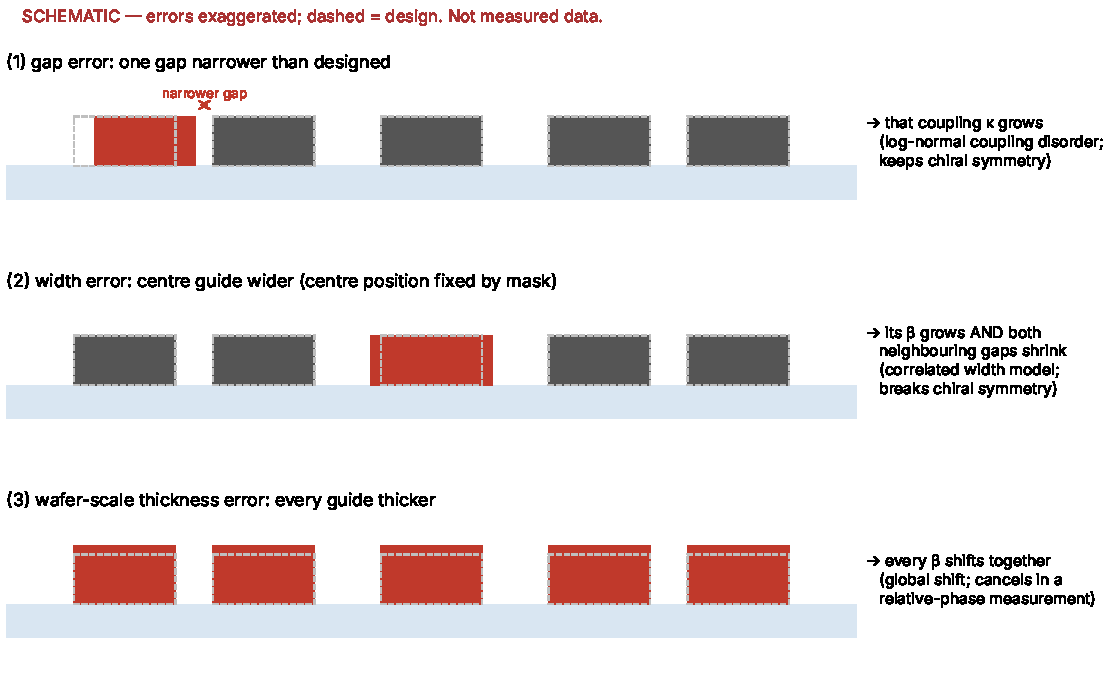
\includegraphics[width=0.9\linewidth]{../../figures/fig_error_schematic.pdf}
\caption{\textbf{Schematic drawn by us} (errors exaggerated; dashed outlines = design). How the three error types of the Monte Carlo map onto a real silicon array of Blanco-Redondo-type dimensions ($450\times220$~nm). Not measured data.}
\end{figure}

\textbf{Real fabrication variation (published images shown in our chat; look these up and cite them, do not copy them as ours):}
\begin{itemize}[itemsep=1pt]
\item \textbf{Wafer-scale maps} of silicon-layer thickness on 300~mm SOI wafers (ellipsometry maps) --- the source of the ``global'' and slowly varying $\beta$ errors.
\item \textbf{SEM images of sidewall roughness} and of directional-coupler gaps that come out different from the design value --- the source of width errors (on-site disorder) and gap errors (coupling disorder).
\item One of the search results is an open-access paper in the MDPI journal \emph{Photonics} on sidewall roughness (MDPI is CC-BY) --- a good candidate for a reusable figure, \emph{after} you check its licence and authors.
\end{itemize}
\textbf{Why this matters for the question Q-ratio:} the published variation data usually report nm of width and thickness variation. Turning those nm into $\sigma_\beta$ and $\sigma_\kappa$ needs $\partial\beta/\partial w$ and $\gamma=\partial\ln\kappa/\partial g$ for the actual waveguide, which needs a mode solver. That is the single most useful optional extension (your COMSOL), because it would turn Fig.~\ref{fig:mc}f into one realistic number.

%=====================================================================
\section{Revised schedule (31 Oct -- 11 Nov)}
%=====================================================================
\begin{tabular}{@{}lll@{}}\toprule
Date & Work & Priority\\\midrule
Sat 31 Oct & Day 4 --- Monte Carlo of $b$ (\textbf{done}) & core\\
Sun 1 Nov & Day 5 --- propagation, phase extraction, loss & core\\
Mon 2 Nov & Day 6 --- Monte Carlo of phase and transmission $\star$ & core\\
Tue 3 Nov & Day 8 --- MZI transfer matrix, mesh, fidelity & core\\
Wed 4 Nov & Days 9--10 --- error propagation and the T-vs-D bridge $\star$ & core\\
Thu 5 Nov & Day 11 --- HOM (two-mode only) & reduced\\
Fri 6 -- Sat 7 Nov & Full paper draft (3--7 pages) & core\\
Sun 8 Nov & Reproducibility + technical audit & core\\
Mon 9 Nov & Viva preparation & core\\
Tue 10 Nov & Buffer & ---\\
Wed 11 Nov & Submit & ---\\\bottomrule
\end{tabular}
\smallskip

The original Day-7 buffer is used up. \textbf{If another day slips:} drop the HOM part to a half-page analytic section (no simulation), then drop the mesh (keep a single MZI).

\section{Code and tests}
New: \texttt{topq/montecarlo.py} (array specs, disordered $H$, mode tracking, ensembles, bootstrap), \texttt{scripts/day4\_mc\_eigen.py}, \texttt{scripts/day4\_error\_schematic.py}, \texttt{tests/test\_montecarlo.py} (7 tests). Whole suite: \textbf{78 passed}.
\textbf{Lesson:} my first test claimed the T mode is pinned ``even when strong'' at $\sigma=0.6$ --- it failed. The failure was real physics (Section 4.2), not a bug. The test now checks what is actually true: a zero mode always exists, but tracking is only guaranteed up to $\sigma=0.3$.

\section{Self-test (answer without notes)}
\begin{enumerate}[itemsep=1pt]
\item Why 2000 samples? What would 200 samples cost you?
\item Why do T and D spread equally under on-site disorder? (One line, using IPR.)
\item The T mode's $b$ does not move under coupling disorder, yet its overlap with the clean mode drops. How is that possible?
\item Why does D's average $b$ go \emph{up}, never down?
\item What single number about real silicon waveguides would decide how useful topological protection is here?
\end{enumerate}
\end{document}
